%*********************************************************************
\chapter{Commissioning and Instrumentation}
\label{ch:commissioning}
%*********************************************************************

Chapter~\ref{ch:design} describes the incubator as designed. This chapter checks that it works, in the same order: the printed enclosure, power and switching, temperature measurement, and the gas sensors. The control loops are not characterised here, since that needs the assembled system and is done in Chapters~\ref{ch:thermalID} and~\ref{ch:ClosedLoop}. The aim is to confirm that every sensor reads correctly, that every actuator can be driven from the STM32, and that the measurement chain is good enough to judge the tolerances in Section~\ref{sec:requirements} against. Every connection referred to below is listed in Appendix~\ref{app:wiring}.

%*********************************************************************
\section{Firmware and Logging}
\label{sec:firmware-settings}
%*********************************************************************

All tests run on the STM32L476RG Nucleo-64, programmed in C++ in PlatformIO with the Arduino framework, chosen for its ready-made sensor libraries and because the loops run every few seconds, so the lower-level control of ST's HAL was not needed. It prints timestamped readings over serial at 115\,200 baud. The ADS1115 runs at the $\pm$4.096\,V gain setting, with each thermistor channel read sixteen times and averaged. The MAX31865 is read in 2-wire mode against its 4300\,$\Omega$ reference. The SCD30 uses its minimum 2\,s interval on an I\textsuperscript{2}C bus clocked at 50\,kHz, since it stretches the clock and is rated to 100\,kHz. The ExplorIR-M is polled over UART at 9600 baud once per second with its filter set to 32. Automatic self-calibration is off on both gas sensors, because both assume regular exposure to fresh air at about 400\,ppm, which a sealed incubator never sees.

Resolution comes from the converters, not the sensors. One ADS1115 step is 0.125\,mV, about 0.003\,\textdegree{}C near 37\,\textdegree{}C, so the thermistor's own tolerance is the limit. One MAX31865 step is $4300/32768 = 0.131$\,$\Omega$, or 0.034\,\textdegree{}C on a PT1000. That bounds every temperature claim in this report.

%*********************************************************************
\section{Printed Enclosure}
\label{sec:build-observations}
%*********************************************************************

The enclosure printed in PETG and went together as designed. The plate sits on its ledge, the lid rib sits in its groove, and the bulkhead fitting and cable gland screw into their holes.

\textbf{It fits the stage.} The base was taken to the laboratory and fitted into the K-frame insert of the open-frame stage it was designed against (Figure~\ref{fig:ch5-built}c, with more views in Appendix~\ref{app:printed-enclosure}). It dropped in and sat flat. This is the result that matters most here, since the fit came from measurements taken by hand and could not be checked any other way.

\begin{figure}[htbp]
    \centering
    \begin{subfigure}[b]{0.31\textwidth}
        \centering
        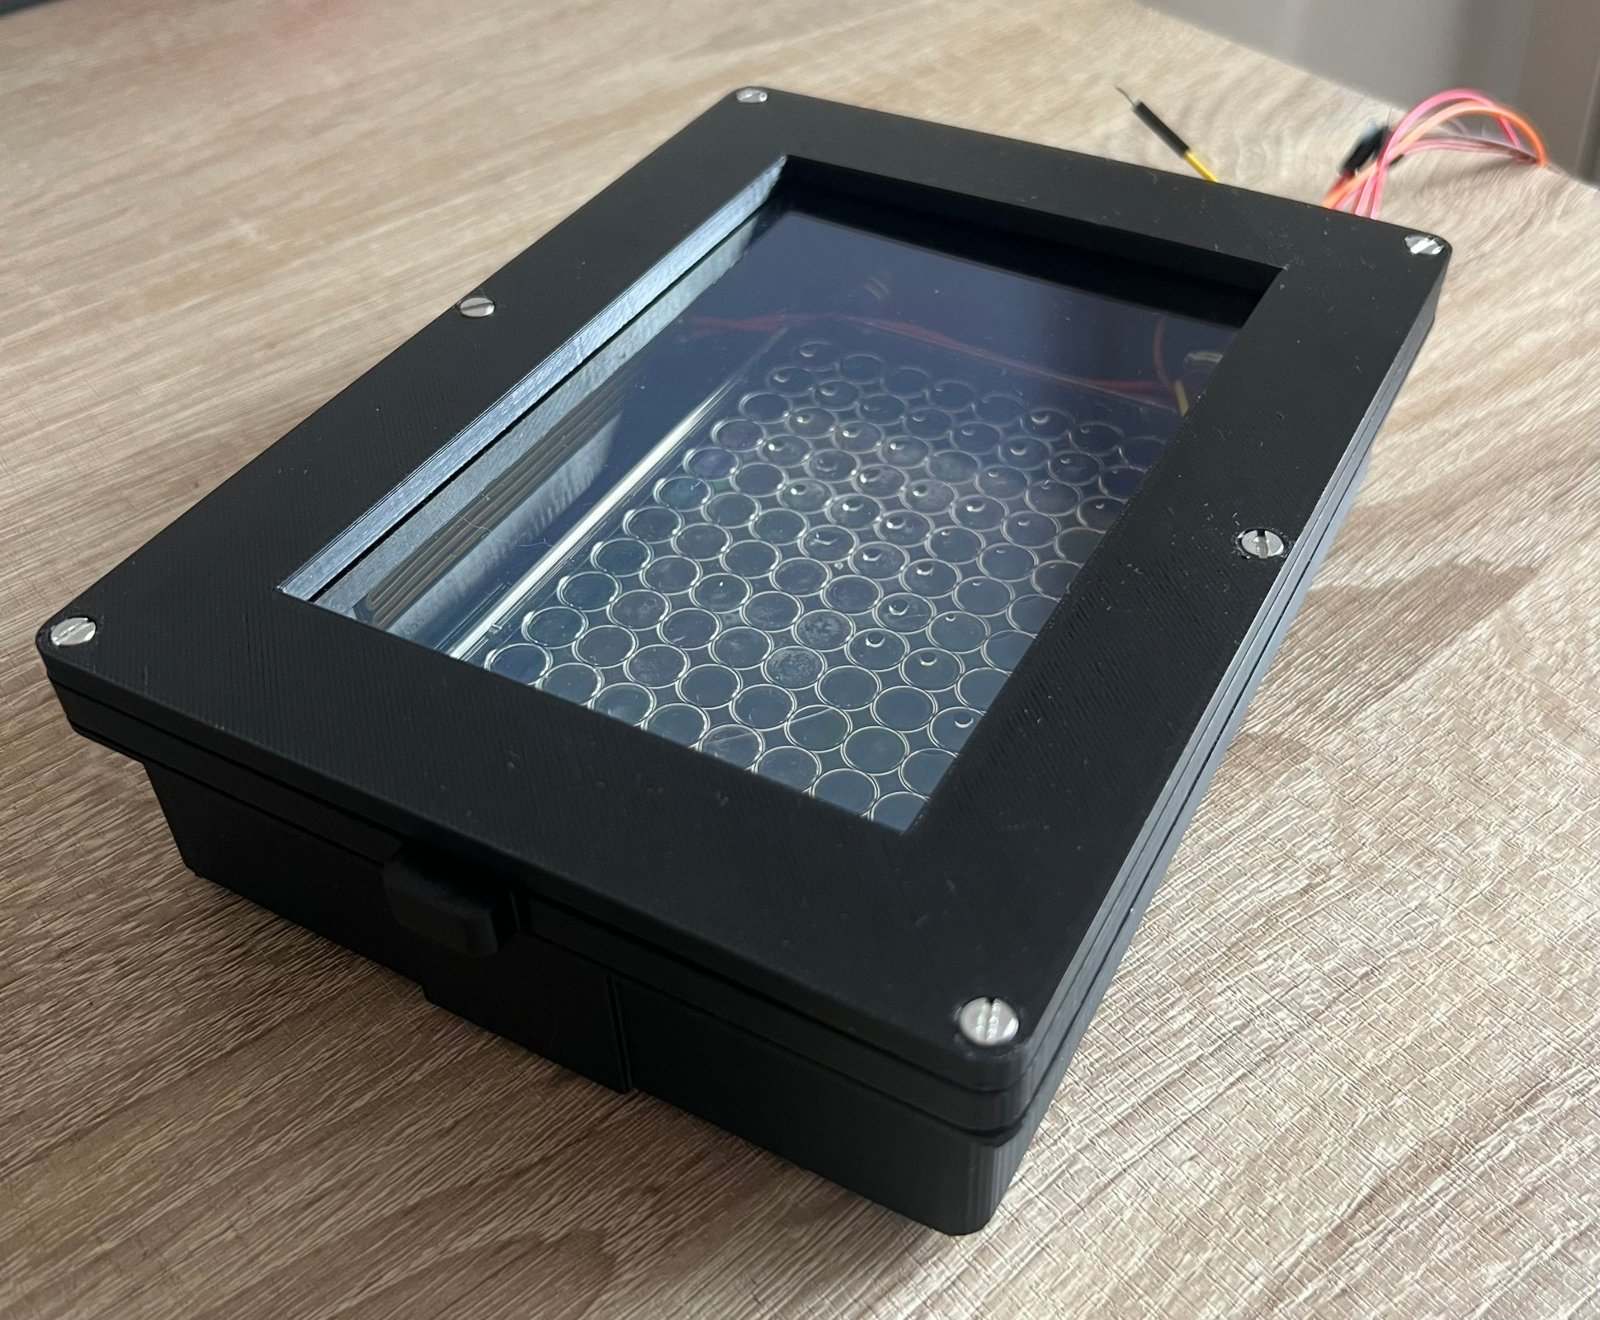
\includegraphics[height=3.2cm]{figs/ch5/enclosure_printed_top.jpg}
        \caption{}
    \end{subfigure}\hfill
    \begin{subfigure}[b]{0.33\textwidth}
        \centering
        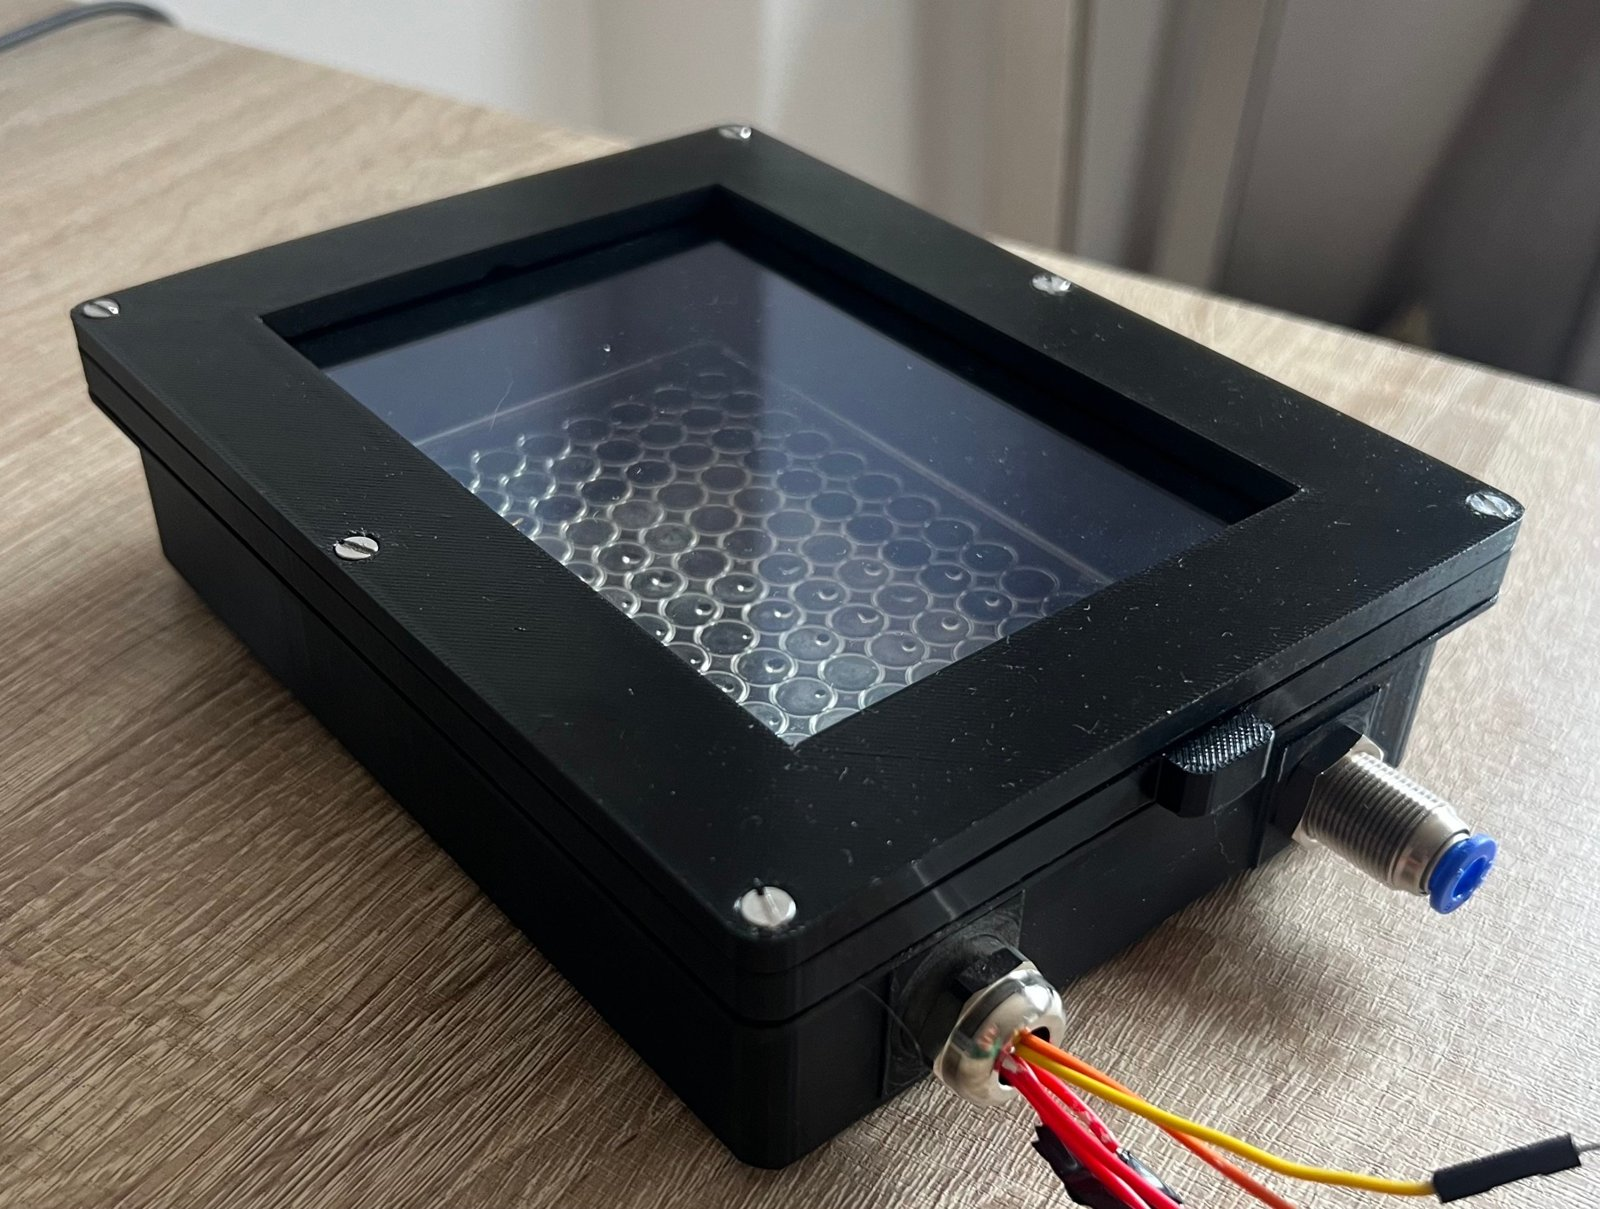
\includegraphics[height=3.2cm]{figs/ch5/enclosure_printed_fittings.jpg}
        \caption{}
    \end{subfigure}\hfill
    \begin{subfigure}[b]{0.33\textwidth}
        \centering
        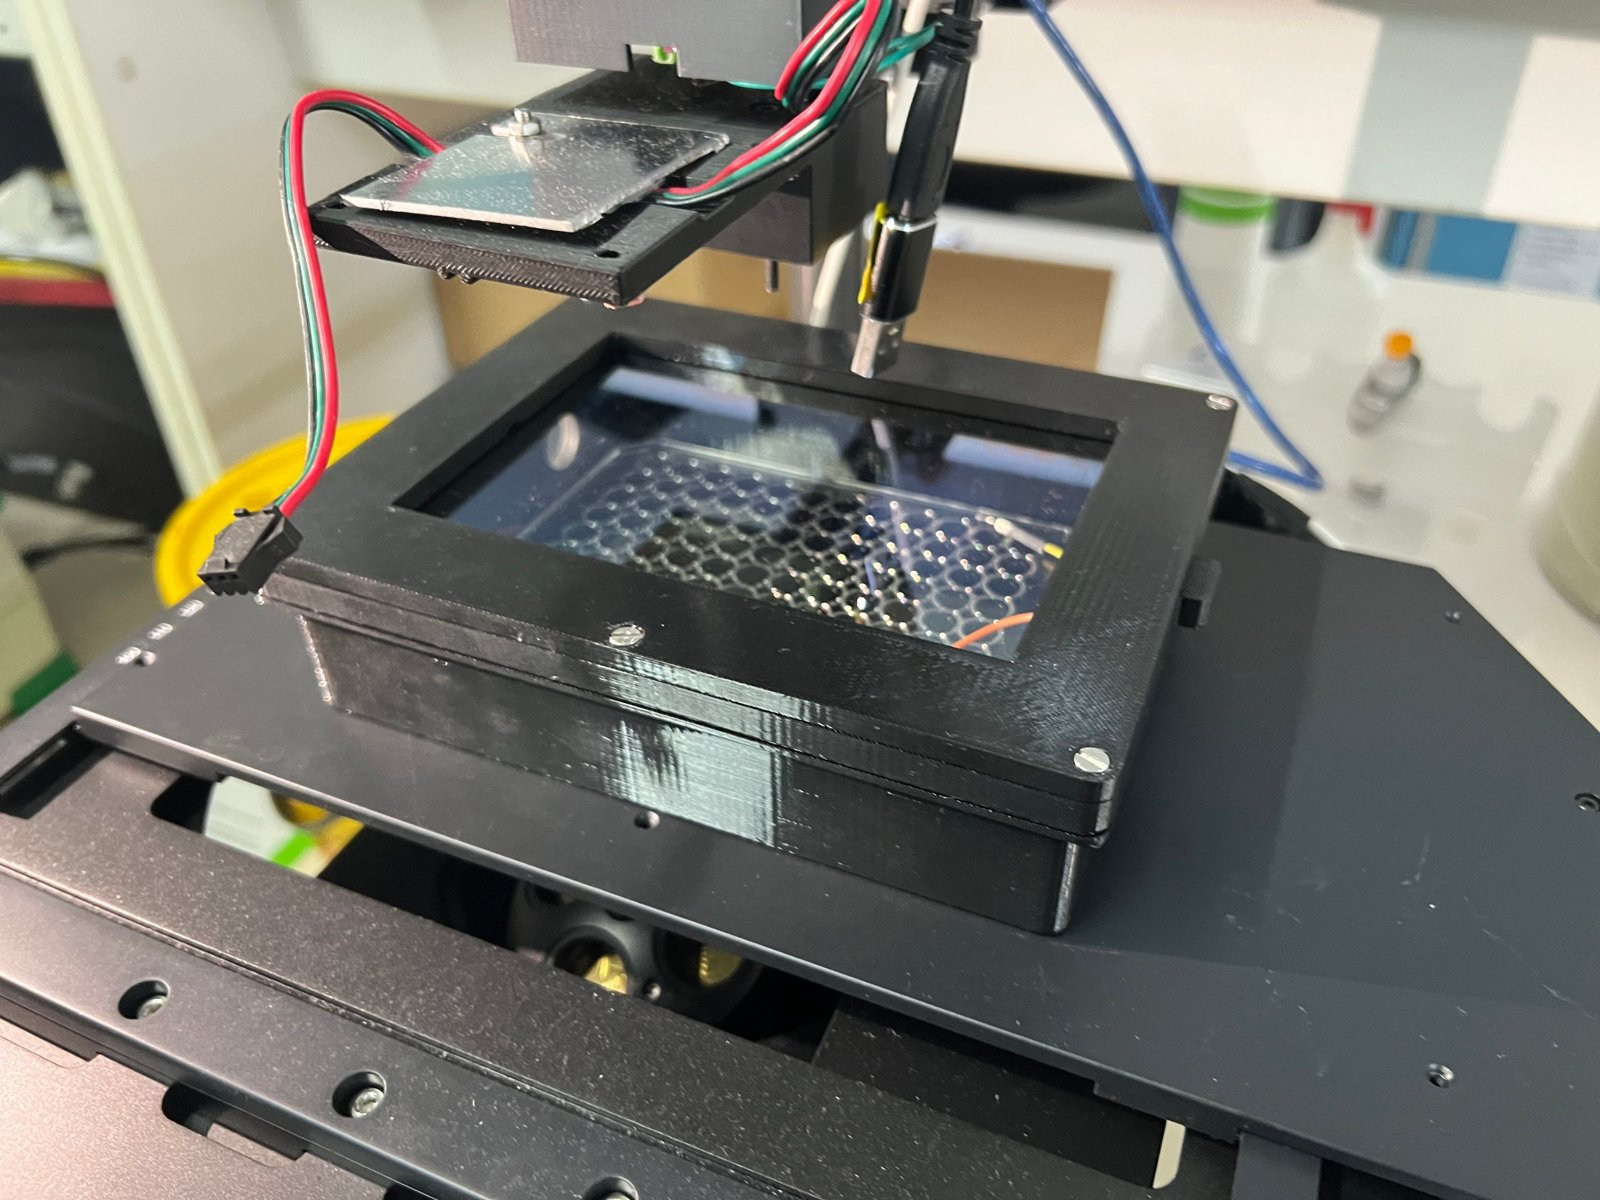
\includegraphics[height=3.2cm]{figs/ch5/enclosure_on_stage_side.jpg}
        \caption{}
    \end{subfigure}
    \caption[The printed enclosure]{\textbf{The printed enclosure.} (a) Assembled, with the plate under the ITO glass lid. (b) The cable gland and gas bulkhead in the end wall. (c) Seated in the K-frame insert of the microscope stage.}
    \label{fig:ch5-built}
\end{figure}

\textbf{A clip snapped.} While the base was being handled on the stage, one of the three plate clips broke off under light thumb pressure through a rubber glove. Section~\ref{sec:enclosure} made the clips thin on purpose, accepting that they might snap, because a plate that will not push past a stiff clip is the worse problem for a first build. That choice was wrong: the clips are too weak to survive handling, let alone repeated plate changes. Thickening them brings back the problem they were made thin to avoid, so they need reinforcing instead. The clip broke at the small notch where it meets the wall, which is the thinnest point and where the bending load concentrates, so removing that notch, adding a rib along the clip and filleting the root would spread the load over a length rather than a line.

Four smaller changes follow from handling the parts. The lid is located by its rib but nothing holds it down, so screws through the lid frame are needed before the incubator is carried anywhere. The seat for the ExplorIR-M is too small and has to be opened up. One 15\,mm cable gland cannot take four thermistors, the PT1000, two gas sensors and the glass heater leads, so a second is needed. And both the 0.8\,mm floor and the 21.9\,mm gap above the plate look larger than they need to be, so the incubator could be made shorter once the clips are stiffened.

%*********************************************************************
\section{Power and Switching}
\label{sec:power-commissioning}
%*********************************************************************

The 12\,V supply measured 12.44\,V, and the buck converter tracked its own display down to 5\,V on a multimeter.

\textbf{Heaters.} Two 12\,V heaters in parallel, about 2\,A total, were switched by the PN2222A and TIP31C pair of Section~\ref{sec:temperature-design}, drawn in Figure~\ref{fig:driver-circuits}a, on a 10\,s on, 20\,s off cycle. The 10\,k$\Omega$ pulldown held them off while the STM32 booted and they followed the cycle exactly. One measurement confirms the concern raised in Chapter~\ref{ch:design}: the TIP31C drops about 2\,V at 2\,A and so dissipates 4\,W, which needs a heatsink for continuous use and is why a logic-level MOSFET is the better second-iteration part.

\textbf{ITO glass.} Copper tape bus bars were applied along the two 112\,mm edges and a wire soldered to each. The resistance between them measured 12.4\,$\Omega$, consistent with the specified 5 to 10\,$\Omega$/sq over this geometry. At 12\,V the panel drew about 1\,A for 11.6\,W and heated evenly over a few minutes, with no hot spots and no contact problems at the tape. That sits inside the 10.7 to 21.5\,W predicted in Section~\ref{subsec:glass-model}.

\begin{figure}[htbp]
    \centering
    \begin{subfigure}[b]{0.58\textwidth}
        \centering
        \begin{circuitikz}[american, scale=0.75, transform shape]
            \ctikzset{bipoles/length=0.9cm}
            \node[npn] (Q1) at (3,2) {};
            \node[npn] (Q2) at (6.5,2) {};
            \node[above left] at (Q1.C) {PN2222A};
            \node[above right] at (Q2.C) {TIP31C};
            \draw (Q1.C) -- (3,4) -- (6.5,4);
            \draw (Q2.C) -- (6.5,4);
            \draw (6.5,4) to[R, l=Heater] (6.5,5.6);
            \draw (6.5,5.6) -- (7.8,5.6) node[right] {$+12$\,V};
            \draw (Q1.E) -- (3,0.9) -- (5.9,0.9) -- (5.9,2) -- (Q2.B);
            \node[circ] at (4.4,0.9) {};
            \draw (4.4,0.9) to[R, l=$1\,\mathrm{k}\Omega$] (4.4,0);
            \draw (Q1.B) to[R, l_=$150\,\Omega$] ++(-2.2,0) node[left] {PWM};
            \draw (Q1.B) -- (2.1,2);
            \node[circ] at (2.1,2) {};
            \draw (2.1,2) to[R, l=$10\,\mathrm{k}\Omega$] (2.1,0);
            \draw (Q2.E) -- (6.5,0);
            \draw (1.6,0) -- (7.8,0);
            \draw (4.9,0) node[ground] {};
        \end{circuitikz}
        \caption{}
        \label{fig:driver-heater}
    \end{subfigure}\hfill
    \begin{subfigure}[b]{0.32\textwidth}
        \centering
        \begin{circuitikz}[american, scale=0.75, transform shape]
            \ctikzset{bipoles/length=0.9cm}
            \draw (0,4.6) node[above] {$+3.3$\,V} -- (0,4.6)
                  to[R, l=$R_\mathrm{fixed}$] (0,2.8)
                  to[thR, l=NTC] (0,0.6);
            \draw (0,0.6) -- (0,0) node[ground] {};
            \draw (0,2.8) -- (1.9,2.8) node[right] {A$n$};
            \node[circ] at (0,2.8) {};
        \end{circuitikz}
        \caption{}
        \label{fig:driver-divider}
    \end{subfigure}
    \caption[Heater driver and thermistor divider]{\textbf{The two circuits that are not module-to-module connections.} (a) One heater channel. The STM32 cannot supply the base current a TIP31C needs at 2\,A, so a PN2222A drives it as a Darlington pair. The 10\,k$\Omega$ holds the heater off while the STM32 boots and the 1\,k$\Omega$ gives a clean turn-off. One channel is built per heated zone. (b) One thermistor channel. Each NTC sits in a divider with its own fixed resistor, measured individually and listed in Table~\ref{tab:wiring}, and the midpoint goes to one ADS1115 input.}
    \label{fig:driver-circuits}
\end{figure}

\textbf{Solenoid.} The relay module turned on and stayed on, because it is low-trigger and the STM32's 3.3\,V logic high is not high enough to release it. Setting the pin to open-drain fixed this: it pulls the input to ground to switch on and releases it to switch off, letting the module pull its own input to 5\,V. With the relay in series with the brown conductor of the solenoid's mains lead, and the mains landed on the normally open contact so no terminal is live while the solenoid is off, the solenoid clicked on and off in step with the STM32. The relay and its mains wiring stayed inside a closed plastic container throughout.

%*********************************************************************
\section{Temperature Measurement}
\label{sec:temperature-commissioning}
%*********************************************************************

Section~\ref{sec:temperature-design} makes one PT1000 the reference and four thermistors the measuring sensors, so commissioning is three steps: get the reference working, measure how far each thermistor sits from it, and confirm that correcting those offsets brings them into line.

\subsection{Reference channel}
\label{subsec:pt1000-commissioning}

The MAX31865 initially returned a fixed $-242.02$\,\textdegree{}C with a raw value of zero, while the PT1000 itself measured about 1085\,$\Omega$ on a multimeter, so the sensor was not the problem. A threshold register written at startup read back as zero, which showed the chip was not responding over SPI at all. The board's 3.3\,V regulator output measured 0.6\,V with 5\,V on VIN, and unpowered the resistance from 3V3 to ground was 35\,$\Omega$ against several k$\Omega$ on a healthy board. An earlier reversed supply connection had shorted the regulator, which the board has no protection against. Removing the regulator restored a high resistance, and since the MAX31865 runs on 3.0 to 3.6\,V the board was powered from the Nucleo's 3.3\,V rail instead. Writing two distinctive values to the fault threshold registers and reading them back returned both correctly, confirming the chip had survived.

\textbf{Ice bath.} Because the board had been through reverse power and rework, the channel was checked against a fixed point. A mixture of ice and water in equilibrium sits at 0\,\textdegree{}C, so it is a reference that comes from physics rather than from another instrument. The first bath used ice cubes and a little cold water and settled at 1001.15\,$\Omega$ and $+0.29$\,\textdegree{}C. That result has two possible causes which the test cannot separate, because both read high: cubes floating in water leave channels of water above 0\,\textdegree{}C, and lead resistance in a 2-wire connection is counted by the converter as part of the sensor. The test was therefore repeated with crushed and drained ice packed densely into an insulated container, and settled at 1001.02\,$\Omega$ and $+0.26$\,\textdegree{}C with a standard deviation of 0.023\,\textdegree{}C. The two baths agree to 0.03\,\textdegree{}C, less than one converter step, even though one was made carelessly and the other carefully, so the ice was not what caused the offset. Appendix~\ref{app:icebath} gives both runs in full.

What remains is 1.02\,$\Omega$ of extra series resistance, which at 0.26\,\textdegree{}C per ohm on a PT1000 accounts for all of it. That is the lead resistance of the 2-wire connection and its contacts, and it is the cost Section~\ref{sec:temperature-design} accepted in choosing a short 2-wire PT1000 over a bulkier 3-wire PT100 that would not fit the chamber.

\textbf{Correction.} A fixed $-0.26$\,\textdegree{}C is applied in firmware, and it cannot be applied to the PT1000 alone. The thermistor offsets below were measured against the uncorrected PT1000, so all four inherit the same bias and correcting only the reference would leave them 0.26\,\textdegree{}C high. The same $-0.26$\,\textdegree{}C is therefore subtracted from all five channels. It changes nothing about how the sensors agree with each other, but it is the difference between the chamber sitting at 37.0\,\textdegree{}C when the firmware reports 37.0 and sitting at 36.74\,\textdegree{}C, which would spend all of R1 before the controller has done anything. The calibration is single-point, and because lead resistance is a fixed resistance rather than a fixed temperature error its effect in degrees is slightly smaller at 37\,\textdegree{}C than at 0\,\textdegree{}C.

\subsection{Thermistor agreement}
\label{subsec:thermistor-commissioning}

Each thermistor sits in a voltage divider with its own fixed resistor, and the ADS1115 measures the midpoint (Figure~\ref{fig:driver-circuits}b). The firmware converts that voltage back to a resistance with the divider equation, then to a temperature with the Beta equation, using the datasheet values of 10\,k$\Omega$ at 25\,\textdegree{}C and $\beta = 3976$\,K. Both steps depend on the fixed resistor and the supply voltage, and a 1\% resistor error alone is about $\pm$0.2\,\textdegree{}C, as large as the thermistor's own tolerance. Each fixed resistor was therefore measured individually and the 3V3 rail measured at 3.29\,V, and those values used in the firmware rather than the nominal ones (Appendix~\ref{app:wiring}).

The four thermistors were first grouped in the same air and logged for three minutes with no reference. All four rose and fell together by up to about 1\,\textdegree{}C as the room air moved, confirming they track the same air at the same speed. Relative to the mean of the four, T1 sat 0.06\,\textdegree{}C low, T3 and T4 about 0.2\,\textdegree{}C high and T2 0.36\,\textdegree{}C low. That shows how they compare but not which is right, which is what the PT1000 is for.

All five were then logged together for six minutes at one reading per second. The PT1000 was steady at a standard deviation of 0.04\,\textdegree{}C while the thermistors fluctuated by about 0.21\,\textdegree{}C, because the small beads respond to air movement within seconds where the larger sheathed probe averages it out. Offsets were therefore taken as averages over the whole run. The mean offsets from the PT1000 were $+0.06$, $-0.51$, $+0.25$ and $+0.23$\,\textdegree{}C for T1 to T4, Each thermistor is rated to $\pm$0.2\,\textdegree{}C \citep{te_ga10k_2019}, so T2, T3 and T4 all sat outside that rating before correction, T2 by the widest margin.

Each offset was applied as a fixed correction in firmware and the test repeated under the same conditions (Figure~\ref{fig:ch5-thermistors}). All four then agree with the PT1000 to within 0.09\,\textdegree{}C and with each other to within 0.02\,\textdegree{}C on average, and the instantaneous spread between them falls from 0.77 to 0.09\,\textdegree{}C. A shared offset of about $-0.07$\,\textdegree{}C remains, but it changed over the run and affects all four equally, so it is the room temperature moving while the PT1000 lags rather than a calibration error.

\begin{figure}[htbp]
    \centering
    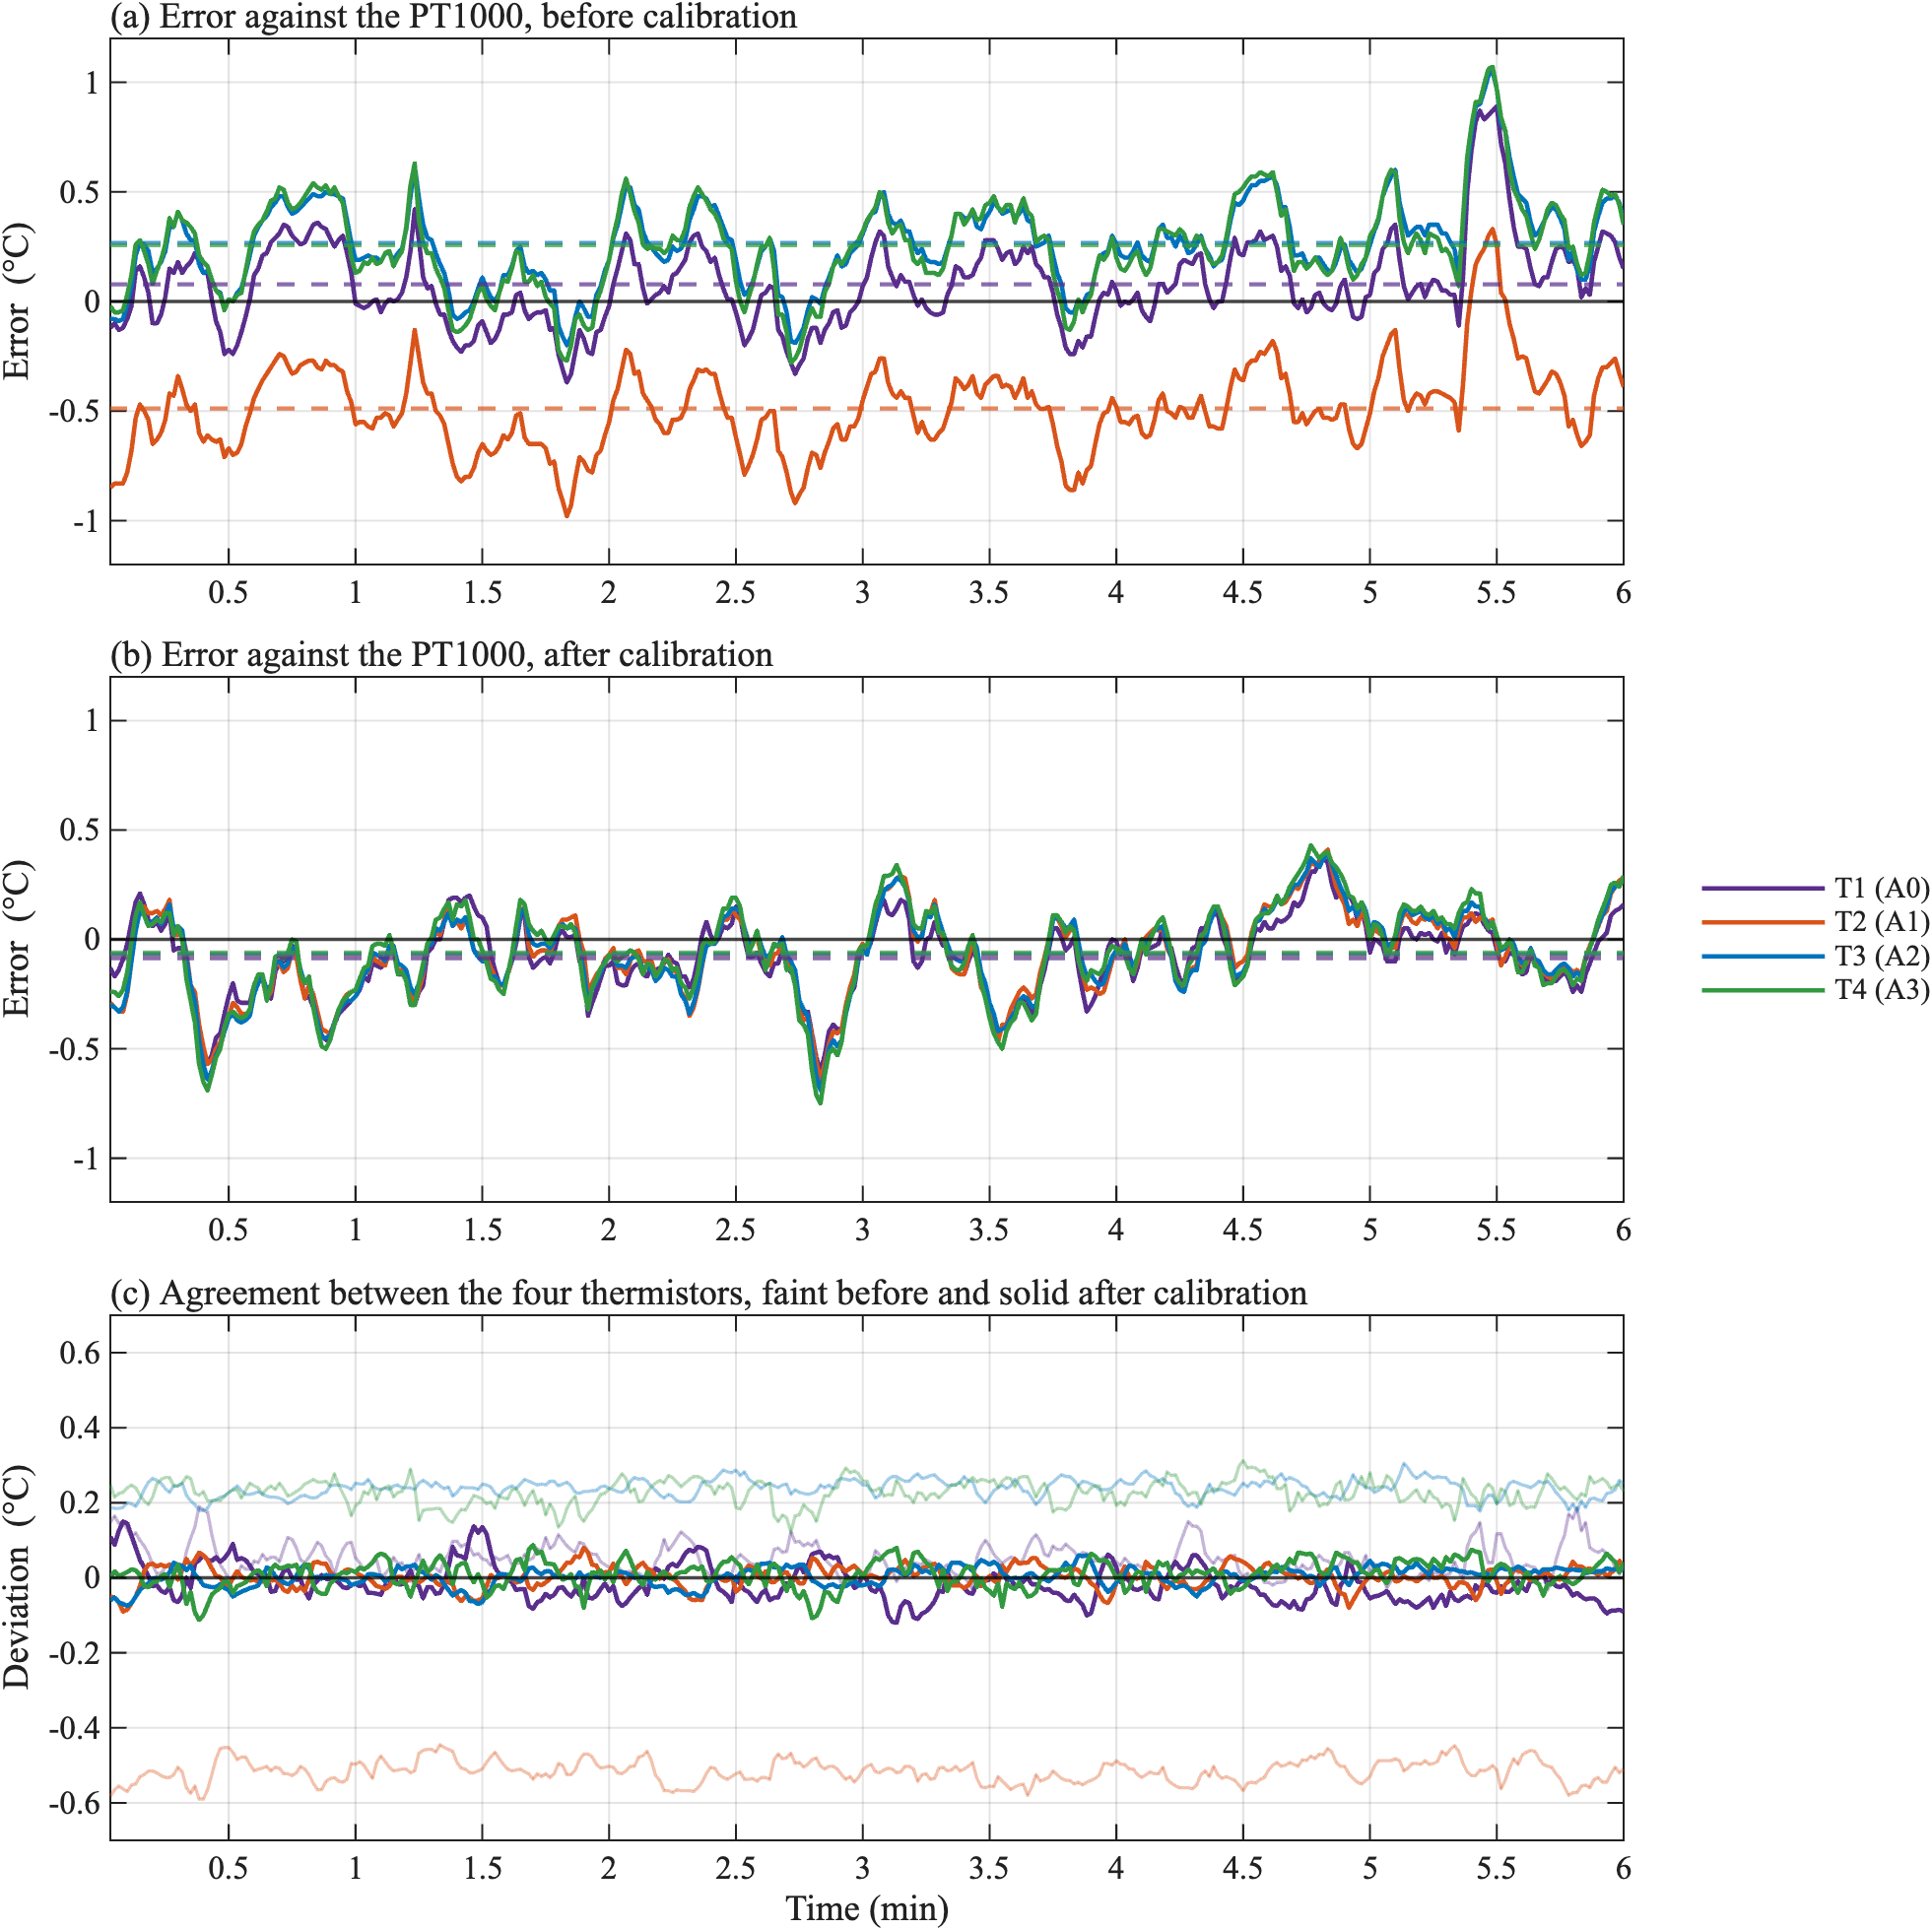
\includegraphics[width=0.70\textwidth,height=0.36\textheight,keepaspectratio]{figs/ch5/fig_M1_thermistor_calibration.png}
    \caption[Thermistor calibration against the PT1000]{\textbf{Thermistor calibration against the PT1000.} (a) and (b) Each thermistor's error against the PT1000, before and after the firmware offsets, with each channel's mean dashed. The common $\pm$0.5\,\textdegree{}C wander is the room moving while the larger PT1000 lags the small beads, so it affects all four equally. (c) Deviation from the mean of the four, faint before and solid after; the worst falls from 0.59 to 0.15\,\textdegree{}C.}
    \label{fig:ch5-thermistors}
\end{figure}

Two limits carry forward. All five sensors share the PT1000's $+0.26$\,\textdegree{}C lead-resistance bias, so relative agreement is better than absolute accuracy. And the offsets were measured at about 23.6\,\textdegree{}C, so they should be rechecked at 37\,\textdegree{}C, since a thermistor's offset shifts with temperature if its Beta differs from the datasheet.

\subsection{Common-mode offset from grounding}
\label{subsec:ground-fault}

During one run all four thermistor channels jumped by about 4\,\textdegree{}C at once and stayed there. A shift on every channel at the same instant cannot be the thermistors, since four independent beads do not change together, and it is far larger than any plausible resistor or supply error. It was traced to the grounding of the measurement side, and moving the ground connection removed it.

%*********************************************************************
\section{Gas and Humidity Sensing}
\label{sec:gas-commissioning}
%*********************************************************************

\textbf{ExplorIR-M zero.} The sensor communicated on the first attempt but read a steady 2000\,ppm indoors, where normal indoor air is 400 to 1000\,ppm, and 1100 to 1200\,ppm outside, where it is about 420\,ppm. It was responding to real changes, dropping by about 900\,ppm between the two, so this was a zero offset rather than a fault. Offsets like this are normal in a new NDIR sensor, since the source and detector drift during shipping and storage.

The datasheet's fresh air procedure was followed: the sensor was powered up outside, sheltered from wind and kept away from people, left to reach a stable temperature with the filter set to 32, and zeroed once the reading had held for a minute. Indoors it then read a steady 500 to 600\,ppm. The readings move in 100\,ppm steps because the 0 to 100\% version reports a raw count scaled by 100, which is the resolution penalty of choosing a sensor that reads past the setpoint. This corrects the offset at 400\,ppm only and does not check the gain.

\textbf{Response.} Breathing on the sensor took it from 500 to 1600\,ppm in about 10\,s and back to baseline about 65\,s after the peak (Figure~\ref{fig:ch5-gas}). The fast rise and slow decay come from CO\textsubscript{2} diffusing back out of the sensor chamber and from the heavy filter, and both are acceptable where CO\textsubscript{2} changes over minutes. The SCD30 behaved the same way on the same test, rising from 593 to 2117\,ppm and recovering to within 10\,ppm of its starting value, with humidity rising from 54\% to 73\%.

\textbf{SCD30 accuracy.} The SCD30 was run indoors at about 665\,ppm and carried outside for seven minutes. After a transient dip it settled at 403\,ppm over the last five minutes, ranging 393 to 413\,ppm (Figure~\ref{fig:ch5-gas}). Typical outdoor CO\textsubscript{2} is 400 to 420\,ppm, so it reads correctly out of the box, inside its $\pm$(30\,ppm $+$ 3\%) specification and with no recalibration. This also confirms the 400\,ppm assumption behind the ExplorIR-M zero, using a second sensor that was never zeroed against it.

\begin{figure}[htbp]
    \centering
    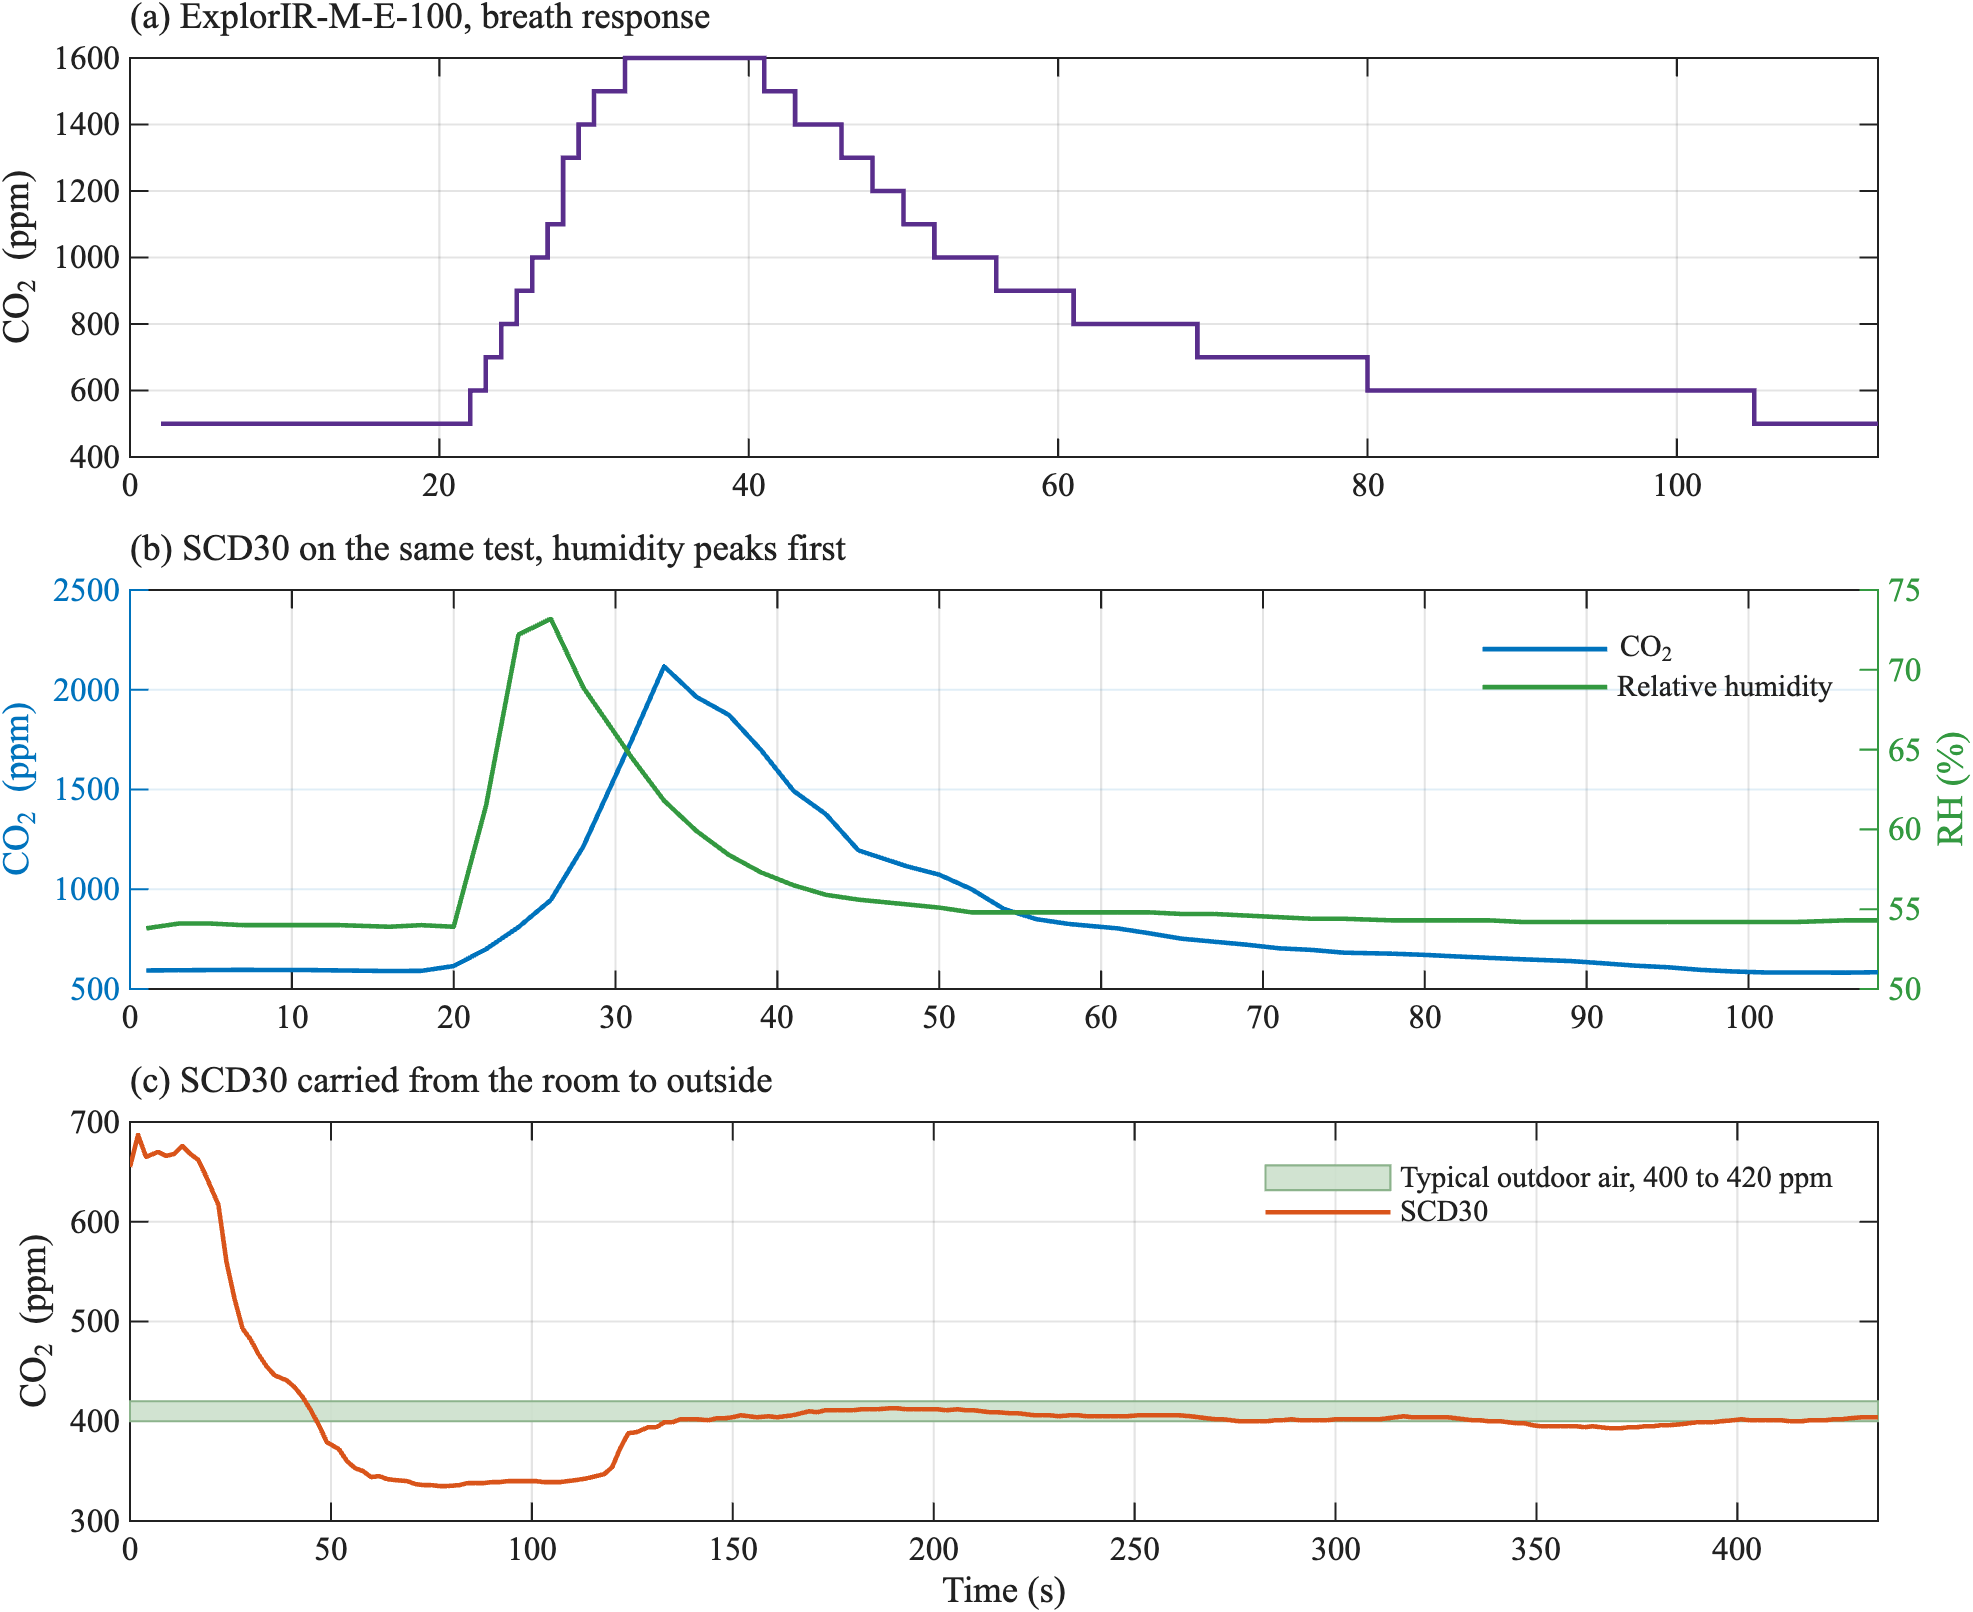
\includegraphics[width=0.68\textwidth]{figs/ch5/fig_M3_gas_sensors.png}
    \caption[Gas sensor commissioning]{\textbf{Gas sensor commissioning.} (a) ExplorIR-M-E-100 responding to breath; the 100\,ppm steps are the resolution of the 0 to 100\% version. (b) The SCD30 on the same test, its humidity channel peaking before the CO\textsubscript{2}. (c) The SCD30 carried outside, settling at 403\,ppm against the typical outdoor band.}
    \label{fig:ch5-gas}
\end{figure}

\textbf{Humidity.} The SCD30's humidity channel responds correctly, rising from 54\% to 73\% during the breath test and returning to its starting value. Its accuracy is taken from the datasheet, $\pm$3\% RH across the full 0 to 100\% range with a drift below 0.25\% RH per year \citep{sensirion_scd30_2020}, and was not verified independently. A saturated salt solution would have given a fixed reference to check it against \citep{greenspan_humidity_1977} and was attempted, but no container was available that sealed properly and the sensor's wires had to pass out through the lid, so room air kept leaking in and the reading never settled.

%*********************************************************************
\section{Summary}
\label{sec:commissioning-summary}
%*********************************************************************

The enclosure fits the stage it was designed against, and every subsystem in Chapter~\ref{ch:design} has been driven from the STM32 with every sensor reading correctly. The one proven fault is the plate clips, one of which snapped during handling. The TIP31C dissipation and the relay's logic level are the two findings that changed how the hardware is driven. The temperature chain resolves to 0.034\,\textdegree{}C and the four thermistors agree with the PT1000 to within 0.09\,\textdegree{}C, well inside the $\pm$0.3\,\textdegree{}C of R1, which makes that requirement testable. The reference reads 0.26\,\textdegree{}C high from lead resistance, which is corrected on all five channels.

Three limits apply to the measurements in the chapters that follow. The ExplorIR-M was zeroed at 400\,ppm and its gain was not checked, so the error quoted at the 5\% setpoint is the datasheet figure rather than a measured one. The temperature calibration used one fixed point at 0\,\textdegree{}C with the thermistor offsets taken at room temperature, so the agreement in Section~\ref{subsec:thermistor-commissioning} is demonstrated well below 37\,\textdegree{}C. And the SCD30's humidity channel was not checked against a reference, so its accuracy rests on the factory calibration.

%*********************************************************************
% End of Commissioning and Instrumentation
%*********************************************************************